
\chapter{Experiments}
In this section, we describe the implementation details and the experimental results obtained after running the benchmark tests. This helps us evaluating the effectiveness of this technique.

\section{Experimental Setup}
All the experiments are performed on a 64-bit Intel Xeon processor with little-endian architecture and x86 instruction set. Fedora 28 is used as an operating system with kernal version 5.0.9-100.fc28.x86\_64. It is to be noted that Java is needed to install the Ghidra software as shown in the documentation \citep{ghidrainstallation}. Ghidra script is written using python and GNU compiler collection is required for running PIN software, designing the Pintool and for the benchmark suite. The implementation details with version information are shown in \cref{tab:table41}.\\
\begin{table}[ht]
\centering\small
\begin{tabularx}{\linewidth}{lX}
\toprule
Tool & Version Details\\
\midrule
Operating System & Fedora release 28\\
Kernel version & 5.0.9-100.fc28.x86\_64\\
GNU compiler collection (gcc and g++) & 8.3.1\\
Intel PIN & pin-3.7-97619-0d0c92f4f\\
Ghidra & 9.0.3-DEV\\
Java JDK & 11.0.2\\
Python & 2.7\\
\bottomrule
\end{tabularx}
\caption{Implementation Details\label{tab:table41}}
\end{table}

To test our implementation, we used SARD - 81 and SARD - 89 test suites (Refer - \citep{black2017sard} \citep{sardcite}) and our own test cases. SARD - 81 has 5 cases and all of them are with buffer overflows. SARD - 89 suite has 291 cases, each having a combination of tests with and without buffer overflows (1164 cases in total). These test cases manifests the vulnerabilities including CWE-119 \citep{cwe119} and CWE-121 \citep{cwe121}. CWE-119 being the top weakness in the "2019 CWE Top 25 Most Dangerous Software Errors"\citep{2019cwetop25} list. We have also created about 50 test cases with overflows, but we do not include those in the results, as those test cases are not standardized. SARD cases consist of buffer overflows with and without using library functions. Note that these test cases only consist of \texttt{C} programs.

\section{Overflow Detection}
In this section, we will discuss about the detection effectiveness of our technique. The end goal of this work is to detect all kinds of memory errors, including spatial memory errors and temporal memory errors. Currently, our technique is focused on providing spatial safety, as discussed earlier. We tested our implementation using SARD benchmarks as discussed before. In case of SARD - 81 benchmark suit, 2 out of 5 tests are passed and in case of SARD - 89 suit, 664 out of 1164 tests are passed. This can be visualized from figures \cref{fig:fig41} and \cref{fig:fig42}. Hence, about 57\% test cases are passed. It should be recalled that all the test cases in SARD - 81 suit show buffer overflows, but SARD - 89 has a combination of tests with and without buffer overflows. 291 of 1169 (i.e. 5 from SARD - 81 and 1164 from SARD - 89) test cases are without overflows. The cases with buffer overflow include overflow by small, medium and large quantity. Also, these cases consist of buffer overflows using library functions, for e.g. using malloc and without using library functions, for e.g. using arrays.

\begin{table}[ht]
\centering\small
\begin{tabularx}{\linewidth}{lX}
\toprule
Reason & Number of Test Cases\\
\midrule
Ghidra script failed to detect & 446\\
Pintool failed to detect & 9\\
String copy (strcpy and strncpy) functions & 25\\
Shared memory Operation (shmat) function & 4\\
Get current working directory (getcwd) function & 3\\
Copy memory area (memcpy) function  & 12\\
Threading & 4\\
\bottomrule
\end{tabularx}
\caption{Case Failure Details (SARD - 81 and SARD - 89)\label{tab:table42}}
\end{table}

\begin{figure}
\begin{centering}
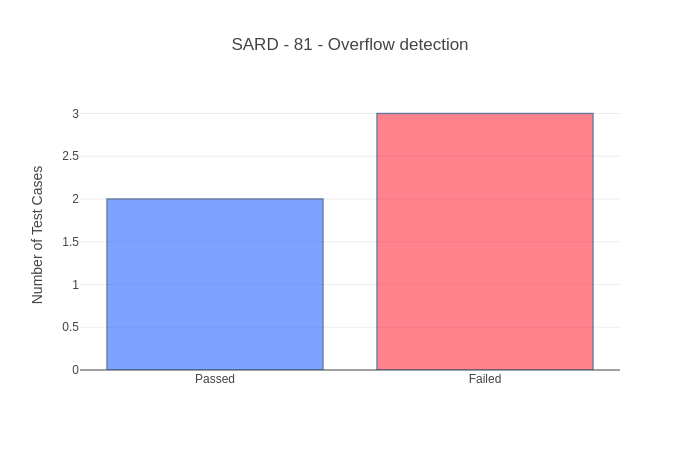
\includegraphics[width=140mm]{images/sard81.png}
\caption{Overflow Detection - SARD - 81\label{fig:fig41}}
\par\end{centering}
\end{figure}

\begin{figure}
\begin{centering}
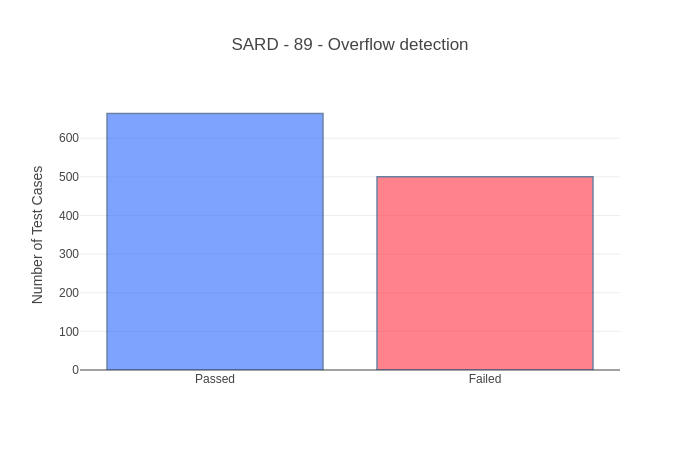
\includegraphics[width=140mm]{images/sard89.png}
\caption{Overflow Detection - SARD - 89\label{fig:fig42}}
\par\end{centering}
\end{figure}

\cref{tab:table42} shows reasons of case failures and the number of failed cases per reason for both SARD - 81 and SARD - 89 benchmarks (i.e. considering 1169 cases in total). Overflows using library functions such as strcpy, strncpy, shmat, getcwd, memcpy are undetected, as library functions are not currently supported (although we manually detect malloc, calloc, realloc, fgets, gets and free). Multi threading is not yet supported and we keep this as a future work. Pintool failed to detect 9 of the cases. This is because certain instructions or pattern of instructions are not being analysed by our Pintool and this can be avoided by carefully modifying the algorithm for those particular cases and other edge cases that may occur. Lastly, there are 446 cases - a significant amount of cases, that are not detected by Ghidra script (Note that these cases may contain library functions, but there may not be a direct impact of library functions on the detection mechanism). The reasons for that include:
\begin{itemize}
    \item \textbf{The location of array access instruction is not detected.}
    \item \textbf{The location of array access instruction is detected incorrectly.}
    \item \textbf{The owner is not detected.}
    \item \textbf{The owner size is detected incorrectly.}
\end{itemize}
The problems in detecting locations of array accesses occur primarily ("primarily", because we observed this in most of the cases) because Ghidra framework's internal algorithms failed to determine it. This may also happen if our algorithm fails to conduct further analysis at run time. For e.g. consider a \texttt{c} program and corresponding assembly in \cref{fig:fig43}. Looking only at the assembly code, it is difficult to predict if the instruction at location \texttt{4004ee} belongs to array \texttt{b1} or if it belongs to array \texttt{b2}. As seen from the example code, array \texttt{b2} clearly overflows and hence the code prints 1 as an output. For the above code, Ghidra predicts the owner of the location \texttt{4004ee} incorrectly, as \texttt{b1} (i.e. it predicts incorrect instruction owner, consequently affecting our technique). \cref{fig:fig44} gives actual examples from SARD benchmarks (Refer - \citep{black2017sard} \citep{sardcite}), which fail to detect the array access instructions. In the program on the left, the array access instruction is falsely predicted as accessed by a scalar and not by an array (and thus the existence of scalar in the code is predicted falsely). In the program on the right, the array access instruction is not detected and hence no owner is assigned to this instruction, which leads to overflow detection failure. We also observed that the access location is mostly detected if the array is indexed using a variable. The chances of detecting the access locations of overflowed arrays become dimmer if the they are indexed using raw numbers (the ones that overflow). As most of cases in SARD suits are close to the ones shown in \cref{fig:fig44}, the failure percentage is higher than expected. \cref{fig:fig44}, \cref{fig:fig45}, \cref{fig:fig46}, \cref{fig:fig47}, \cref{fig:fig48}, \cref{fig:fig49} and \cref{fig:fig410} show examples of each of the above discussed cases (actual examples from SARD benchmarks (Refer - \citep{black2017sard} \citep{sardcite})).

\begin{figure}
\begin{centering}
\begin{tabular}{ c | c }
\begin{lstlisting}
#include <stdio.h>
int main()
{
  int b1[5];
  int b2[10];
  b2[15] = 1;
  printf("%i\n", b1[3]);
  return 0;
}
\end{lstlisting}
&
\begin{lstlisting}
4004e6 push rbp
4004e7 mov rbp,rsp
4004ea sub rsp,0x50
4004ee mov DWORD PTR [rbp-0x14],0x1
4004f5 mov eax,DWORD PTR [rbp-0x14]
4004f8 mov esi,eax
4004fa mov edi,0x400590
4004ff mov eax,0x0
400504 call 4003f0 <printf@plt>
400509 mov eax,0x0
40050e leave
40050f ret 
\end{lstlisting}
\end{tabular}
\caption{Ambiguous Array Access\label{fig:fig43}}
\par\end{centering}
\end{figure}

\begin{figure}
\begin{centering}
\begin{tabular}{ c | c }
\begin{lstlisting}
int main(int argc, char *argv[])
{
  char buf[10];
  /*  BAD  */
  buf[10] = 'A';
  return 0;
}
\end{lstlisting}
&
\begin{lstlisting}
int main(int argc, char *argv[])
{
  char buf[10];
  /*  BAD  */
  buf[4105] = 'A';
  return 0;
}
\end{lstlisting}
\end{tabular}
\caption{Ghidra Script detection failure (example is Taken from SARD suit~\protect\citep{sardcite})\label{fig:fig44}}
\par\end{centering}
\end{figure}

\begin{figure}
\begin{centering}
\begin{tabular}{ c }
\begin{lstlisting}
int main(int argc, char *argv[])
{
  int i;
  char buf[10];
  i = 9;
  /*  OK  */
  (buf + i)[0] = 'A';
  return 0;
}
\end{lstlisting}
\end{tabular}
\caption{Pintool detection failure (example is Taken from SARD suit~\protect\citep{sardcite})\label{fig:fig45}}
\par\end{centering}
\end{figure}

\begin{figure}
\begin{centering}
\begin{tabular}{ c }
\begin{lstlisting}
#include <string.h>
int main(int argc, char *argv[])
{
  char buf[10];
  /*  BAD  */
  strcpy(buf, "AAAAAAAAAAAAAAAAA");
  return 0;
}
\end{lstlisting}
\end{tabular}
\caption{String Copy (strcpy) (example is Taken from SARD suit~\protect\citep{sardcite})\label{fig:fig46}}
\par\end{centering}
\end{figure}

\begin{figure}
\begin{centering}
\begin{tabular}{ c }
\begin{lstlisting}
#include <sys/types.h>
#include <sys/ipc.h>
#include <sys/shm.h>
#include <assert.h>
#include <stdlib.h>
int getSharedMem()
{
  return (shmget(IPC_PRIVATE, 10, 0xffffffff));
}
void relSharedMem(int memID)
{
  struct shmid_ds temp;
  shmctl(memID, IPC_RMID, &temp);
}
int main(int argc, char *argv[])
{
  int memIdent;
  char * buf;
  memIdent = getSharedMem();
  assert(memIdent != -1);
  buf = ((char *) shmat(memIdent, NULL, 0));
  assert(((int)buf) != -1);
  /*  BAD  */
  buf[17] = 'A';
  shmdt((void *)buf);
  relSharedMem(memIdent);
  return 0;
}
\end{lstlisting}
\end{tabular}
\caption{Shared Memory Operations (shmat) (example is Taken from SARD suit~\protect\citep{sardcite})\label{fig:fig47}}
\par\end{centering}
\end{figure}

\begin{figure}
\begin{centering}
\begin{tabular}{ c }
\begin{lstlisting}
#include <unistd.h>
int main(int argc, char *argv[])
{
  char buf[10];
  /*  BAD  */
  getcwd(buf, 18);
  return 0;
}
\end{lstlisting}
\end{tabular}
\caption{Current working directory (getcwd) (example is Taken from SARD suit~\protect\citep{sardcite})\label{fig:fig48}}
\par\end{centering}
\end{figure}

\begin{figure}
\begin{centering}
\begin{tabular}{ c }
\begin{lstlisting}
#include <string.h>
int main(int argc, char *argv[])
{
  int copy_size;
  char src[4106];
  char buf[10];
  memset(src, 'A', 4106);
  src[4106 - 1] = '\0';
  copy_size = -1;
  if (copy_size <= (int)(sizeof buf))
  {
    /*  BAD  */
    memcpy(buf, src, copy_size);
  }
  return 0;
}
\end{lstlisting}
\end{tabular}
\caption{Copy memory area (memcpy) (example is Taken from SARD suit~\protect\citep{sardcite})\label{fig:fig49}}
\par\end{centering}
\end{figure}

\begin{figure}
\begin{centering}
\begin{tabular}{ c }
\begin{lstlisting}
#include <pthread.h>
void * thread_function1(void * arg1)
{
  char buf[10];
  /*  BAD  */
  buf[4105] = 'A';
  pthread_exit((void *)NULL);
  return 0;
}
int main(int argc, char *argv[])
{
  pthread_t  thread1;
  pthread_create(&thread1, NULL, &thread_function1, (void *)NULL);
  pthread_exit((void *)NULL);
  return 0;
}
\end{lstlisting}
\end{tabular}
\caption{Threading (pthread) (example is Taken from SARD suit~\protect\citep{sardcite})\label{fig:fig410}}
\par\end{centering}
\end{figure}

\section{Run Time Overhead}
The run time overhead is also one of the important factors to determine the effectiveness of the mechanism. We used same benchmark suits (SARD) as mentioned in the previous section, to measure the overhead. \cref{fig:fig411} and \cref{fig:fig412} show overhead analysis of SARD - 81 and SARD - 89 suits (\cref{fig:fig413} shows the zoomed in version of \cref{fig:fig412}). We divide the analysis into 3 different tests - test1, test2 and test3. Where test1 calculates the time taken by raw binary to run (i.e. without any tool), test2 calculates the run time of binary if run using a minimal Pintool (a tool with no instrumentation - \cref{fig:fig415}) and test3 computes the time taken by binary if run using our Pintool. We run each test (test1, test2 and test3) 15 times on all the benchmark cases and took the average of those 15 runs for each case. From \cref{fig:fig411} and \cref{fig:fig412} it can be seen that our tool adds a big amount overhead, although considering the minimal tool's overhead, it can be concluded that significant amount of this overhead incurred by pin framework itself (i.e. PIN startup overhead). \cref{fig:fig414} shows average overhead of the 3 tests. Considering the average overheads, we observed about large overhead, but most of the overhead is PIN startup overhead. It will have a negligible effect if measured against bigger programs, as PIN uses code cache, it doesn't have to translate the frequently executing code. By comparing run times of our implementation and the minimal Pintool example, it can be inferred that our implementation adds about 6.15\% overhead. This is due to the inclusion of instrumentation routines in our tool, unlike the minimal Pintool.

\begin{figure}
\begin{centering}
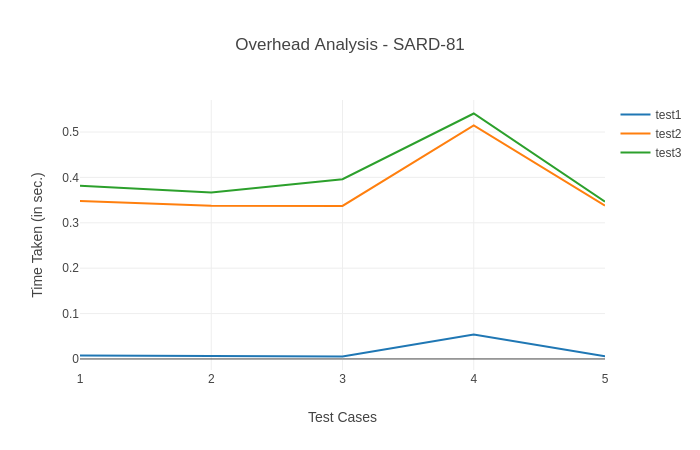
\includegraphics[width=140mm]{images/sard81_overhead.png}
\caption{Overhead Analysis - SARD - 81\label{fig:fig411}}
\par\end{centering}
\end{figure}

\begin{figure}
\begin{centering}
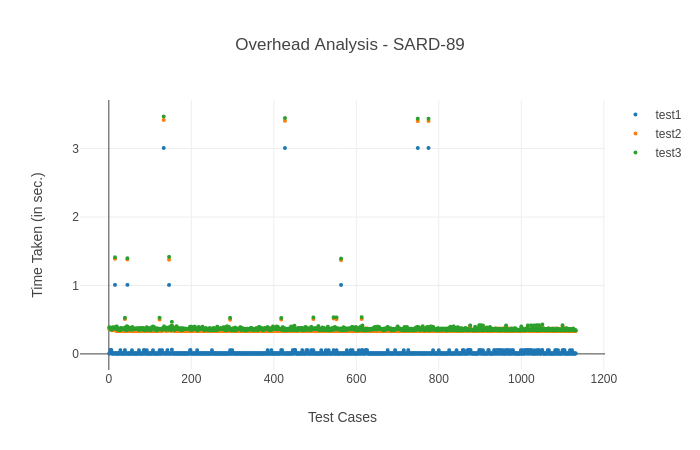
\includegraphics[width=140mm]{images/sard89_overhead.png}
\caption{Overhead Analysis - SARD - 89\label{fig:fig412}}
\par\end{centering}
\end{figure}

\begin{figure}
\begin{centering}
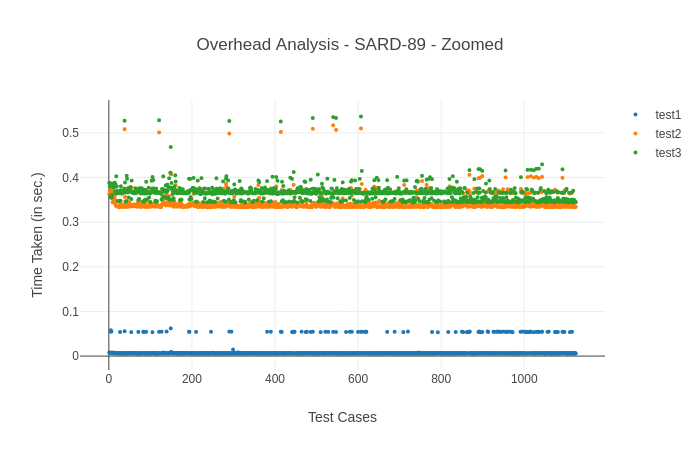
\includegraphics[width=140mm]{images/sard89_overhead_zoomed.png}
\caption{Overhead Analysis - SARD - 89 (zoomed)\label{fig:fig413}}
\par\end{centering}
\end{figure}

\begin{figure}
\begin{centering}
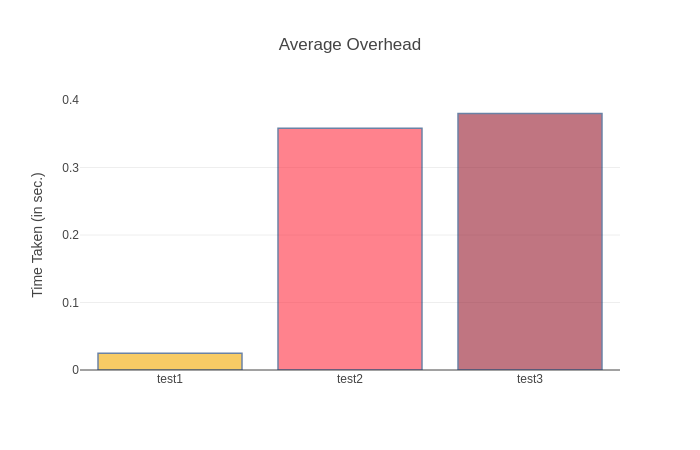
\includegraphics[width=140mm]{images/average_overhead.png}
\caption{Average Overhead\label{fig:fig414}}
\par\end{centering}
\end{figure}

\begin{figure}
\begin{centering}
\begin{tabular}{ c }
\begin{lstlisting}
#include "pin.H"
int main(int argc, char * argv[])
{
    // Initialize pin
    PIN_Init(argc, argv);

    // Start the program, never returns
    PIN_StartProgram();

    return 0;
}
\end{lstlisting}
\end{tabular}
\caption{Minimal Pintool\label{fig:fig415}}
\par\end{centering}
\end{figure}